\section{Computer Networks and the Internet}
\begin{itemize}

\item
When we say a wireless is ``associated'' with a base station, we mean that (1) host is within the wireless communication distance of the base station, and (2) the host uses that base station to relay data between it (the host) and the larger network.

\item
Hosts associated with a base station are often referred to as operating in \textbf{infrastructure mode}, since all traditional network services (e.g., address assignment and routing) are provided by the network to which a host is connected via the base station. In \textbf{ad hoc network}, wireless hosts have no such infrastructure with which to connect. In the absence of such infrastructure, the hosts themselves must provide for services such as routing, address assignment, DNS-like name translation, and more.

\item
Indeed, we can find a number of important differences between a wired link and a wireless link: (1) Decreasing signal strength; (2) Interference from other sources; and (3) Multipath propagation.

\item
The \textbf{signal-to-noise (SNR)} is a relative measure of the strength of the received signal (i.e., the information being transmitted) and this noise.

\item
With the so-called \textbf{hidden terminal problem}, physical obstructions in the environment (for example, a mountain or a building) may prevent A and C from hearing each other's transmissions, even though A's and C's transmissions are indeed interfering at the destination, B. A second scenario that results in undetectable collisions at the receiver results from  the \textbf{fading} of a signal's strength as it propagates through the wireless medium.

\item
In a CDMA protocol, each bit being sent is encoded by multiplying the bit by a signal (the code) that changes at a much faster rate (known as the \textbf{chipping rate}) than the original sequence of data bits.

\item
Although many technologies and standards for wireless LANs were developed in the 1990s, one particular class of standards has clearly emerged as the winner: the \textbf{IEEE 802.11 wireless LAN}, also known as \textbf{WiFi}.

\item
The fundamental building block of the 802.11 architecture is the \textbf{basic service set (BSS)}. A BSS contains one or more wireless stations and a central \textbf{base station}, known as an \textbf{access point (AP)} in 802.11 parlance.\\
When a network administrator installs an AP, the administrator assigns a one- or two-word \textbf{Service Set Identifier (SSID)} to the access point.\\
The administrator must also assign a channel number to the AP. To understand channel numbers, recall that 802.11 operates in the frequency range of 2.4 GHz to 2.485 GHz. Within this 85 MHz band, 802.11 defines 11 partially overlapping channels. Any two channels are non-overlapping if and only if they are separated by four or more channels.

\item
A \textbf{WiFi jungle} is any physical location where a wireless station receives a sufficiently strong signal from two or more APs.

\item
The 802.11 standard requires that an AP periodically send \textbf{beacon frames}, each of which includes the AP's SSID and MAC address. The process of scanning channels and listening for beacon frames is known as \textbf{passive scanning}. A wireless host can also perform \textbf{active scanning}, by broadcasting a probe frame that will be received by all APs within the wireless host's range.

\item
In order to create an association with a particular AP, the wireless station may be required to authenticate itself to the AP. 802.11 wireless LANs provide a number of alternatives for authentication and access. One approach, used by many companies, is to permit access to a wireless network based on station's MAC address. A second approach, used by many Internet caf\'{e}s, employs usernames and passwords. In both cases, the AP typically communicates with an authentication server, relaying information between the wireless end-point station and the authentication server using a protocol such as RADIUS or DIAMETER.

\item
Inspired by the huge success of Ethernet and its random access protocols, the designers of 802.11 chose a random access protocol for 802.11 wireless LANs. This random access protocol is referred to as \textbf{CSMA with collision avoidance}, or more succinctly as \textbf{CSMA/CA}.\\
When the destination station receives a frame that passes the CRC, it waits a short period of time known as the \textbf{Short Inter-frame Spacing (SIFS)} and then sends back an acknowledgement frame.\\
If initially the station senses the channel idle, it transmits its frame after a short period of time known as the \textbf{Distributed Inter-frame Spacing (DIFS)}.\\
In 802.11, if the two stations sense the channel busy, they both immediately enter random backoff, hopefully choosing different backoff values.

\item
In order to avoid the hidden terminals problem, the IEEE 802.11 protocol allows a station to use a short \textbf{Request to Send (RTS)} control frame and a short \textbf{Clear to Send (CTS)} control frame to \textit{reserve} access to the channel.

\begin{figure}[h]
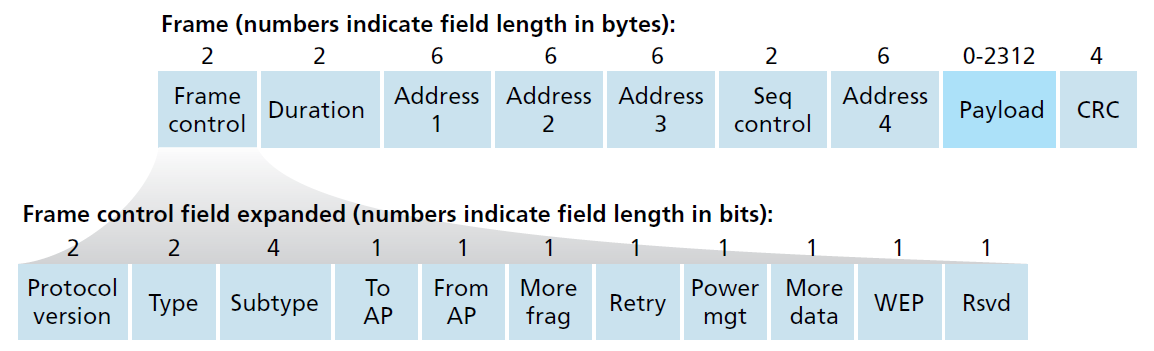
\includegraphics[scale=0.3]{Img-06-01-The-80211-frame}
\centering
\caption{The 802.11 frame}
\label{fig:fig-06-01}
\end{figure}

\item
The 802.11 standard defines the three address fields as follows:
\begin{itemize}
\item[*]Address 2 is the MAC address of the station that transmits the frame.
\item[*]Address 1 is the MAC address of the wireless station that is to receive the frame.
\item[*]To understand address 3, recall that the BSS (consisting of the AP and wireless stations) is part of a subnet, and that this subnet connects to other subnets via some router interface. Address 3 contains the MAC address of this router interface.
\end{itemize}

\item
When the host moves between BSSs in the same subnet, how does the switch know that the host has moved from one AP to another? One solution (a bit of hack, really) is for AP2 to send a broadcast Ethernet frame with H1's source address to the switch just after the new association.

\item
Some 802.11 implementations have a rate adaptation capability that adaptively selects the underlying physical-layer modulation technique to use based on current or recent channel characteristics.

\item
A node is able to explicitly alternate between sleep and wake states. A node indicates to the access point that it will be going to sleep by setting the power-management bit in the header of an 802.11 frame to 1.

\item
Two other IEEE 802 protocols---Bluetooth and Zigbee (defined in the IEEE 802.15.1 and IEEE 802.15.4 standards) and WiMAX (defined in the IEEE 802.16 standard)---are standards for communicating over shorter and longer distances, respectively.

\item
802.15.1 networks operate in the 2.4 GHz unlicensed radio band in a TDM manner, with time slots of 625 microseconds. During each time slot, a sender transmits on one of 79 channels, with the channel changing in a known but pseudorandom manner from slot to slot. This form of channel hopping, known as \textbf{frequency-hopping spread spectrum (FHSS)}, spreads transmissions in time over the frequency spectrum. 802.15.1 can provide data rates up to 4 Mbps.\\
802.15.1 networks are ad hoc networks: No network infrastructure (e.g., an access point) is needed to interconnect 802.15.1 devices. Thus, 802.15.1 devices must organize themselves. 802.15.1 devices are first organized into a \textbf{piconet} of up to eight active devices. One of these devices is designated as the master, with the remaining devices acting as slaves.

\item
While Bluetooth networks provide a ``cable replacement'' data rate of over a Megabit per second, Zigbee is targeted at lower-powered, lower-data-rate, lower-duty-cycle applications than Bluetooth.

\item
In our description of cellular network architecture in this section, we'll adopt the terminology of the \textit{Global System for Mobile Communications (\textbf{GSM})} standards.

\item
The term \textit{cellular} refers to the fact that the region covered by a cellular network is partitioned into a number of geographic coverage areas, known as \textbf{cells}. Each cell contains a \textbf{base transceiver station (BTS)} that transmits signals to and receives signals from the mobile stations in its cell.\\
A GSM network's \textbf{base station controller (BSC)} will typically service several tens of base transceiver stations. The role of the BSC is to allocate BTS radio channels to mobile subscribers, perform \textbf{paging} (finding the cell in which a mobile user is resident), and perform handoff of mobile users. THe base station controller and its controlled base transceiver stations collectively constitute a GSM \textbf{base station system (BSS)}.\\
As we'll see, the \textbf{mobile switching center (MSC)} plays the central role in user authorization and accounting (e.g., determining whether a mobile device is allowed to connect to the cellular network), call establishment and teardown, and handoff.

\item
In our discussion below, we'll focus on the UMTS (Universal Mobile Telecommunications Service) 3G standards developed by the 3rd Generation Partnership Project (3GPP), a widely deployed 3G technology.\\
Given the considerable amount of existing infrastructure (and profitable services!) in the existing cellular voice network, the approach taken by the designers of 3G data services is clear: \textit{leave the existing core GSM cellular voice network untouched}, \textit{adding additional cellular data functionality in parallel to the existing voice network}.\\
There are two types of nodes in the 3G core network: \textbf{Serving GPRS Support Nodes (SGSNs)} and \textbf{Gateway GPRS Support Nodes (GGSNs)}. (GPRS stands for Generalized Packet Radio Service, an early cellular data service in 2G networks; here we discuss the evolved version of GPRS in 3G networks).\\
The 3G \textbf{radio access network} is the wireless first-hop network that we see as a 3G user. The \textbf{Radio Network Controller (RNC)} typically controls several cell base transceiver stations similar to the base stations that we encountered in 2G systems (but officially known in 3G UMTS parlance as a ``Node Bs''---a rather non-descriptive name!).

\item
The 4G Long-Term-Evolution (LTE) standard put forward by the 3GPP has two important innovations over 3G systems: (1) Evolved Packet Core (EPC), and (2) LTE Radio Access Network.\\
An additional 4G wireless technology---WiMAX (World Interoperability for Microwave Access)---is a family of IEEE 802.16 standards that differ significantly from LTE.

\item
In a network setting, the permanent home of a mobile node (such as a laptop or smartphone) is known as the \textbf{home network}, and the entity within the home network that performs the mobility management functions on behalf of the mobile node is known as the \textbf{home agent}. The network in which the mobile node is currently residing is known as the \textbf{foreign} (or \textbf{visited}) \textbf{network}, and the entity within the foreign network that helps the mobile node with the mobility management functions is known as a \textbf{foreign agent}. A \textbf{correspondent} is the entity wishing to communicate with the mobile node.

\item
An alternative approach (and one that has been adopted in practice) is to push mobility functionality from the network core to the network edge. A natural way to do this is via the mobile node's home network.\\
One role of the foreign agent is to create a so-called \textbf{care-of address (COA)} for the mobile node, with the network portion of the COA matching that of the foreign network. A second role of the foreign agent is to inform the home agent that the mobile node is resident in its (the foreign agent's) network and has the given COA.

\item
In the \textbf{indirect routing} approach, the correspondent simply addresses the datagram to the mobile node's permanent address and sends the datagram into the network, blissfully unaware of whether the mobile node is resident in its home network or is visiting a foreign network; mobility is thus completely transparent to the correspondent.\\
\textbf{Direct routing} overcomes the inefficiency of triangle routing, but does so at the cost of additional complexity. In the direct routing approach, a \textbf{correspondent agent} in the correspondent's network first learns the COA of the mobile node. This can be done by having the correspondent agent query the home agent, assuming that (as in the case of indirect routing) the mobile node has an up-to-date value for its COA registered with its home agent.

\item
The Internet architecture and protocols for supporting mobility, collectively known as mobile IP, are defined primarily in RFC 5944 for IPv4.\\
The mobile IP standard consists of three main pieces: (1) Agent discovery; (2) Registration with the home agent; and (3) Indirect routing of datagrams.

\item
Agent discovery can be accomplished in one of two ways: via agent advertisement or via agent solicitation.\\
With \textbf{agent advertisement}, a foreign or home agent advertises its services using an extension to the existing router discovery protocol.\\
With \textbf{agent solicitation}, a mobile node wanting to learn about agents without waiting to receive an agent advertisement can broadcast an agent solicitation message, which is simply an ICMP message with type value 10.

\item
In GSM terminology, the mobile user's home network is referred to as the mobile user's \textbf{home public land mobile network (home PLMN)}.

\item
As in the case of mobile IP, the responsibilities of the home and visited networks are quite different.\\
The home network maintains a database known as the \textbf{home location register (HLR)}, which contains the permanent cell phone number and subscriber profile information for each of its subscribers. As we'll see, a special switch in the home network, known as the \textbf{Gateway Mobile services Switching Center (GMSC)} is contacted by a correspondent when a call is placed to a mobile user.\\
The visited network maintains a database known as the \textbf{visitor location register (VLR)}. The VLR contains an entry for each mobile user that is \textit{currently} in the portion of the network served by the VLR.

\item
While it is associated with a base station, a mobile periodically measures the strength of a beacon signal from its current base station as well as beacon signals from nearby base stations that it can ``hear''. These measurements are reported once or twice a second to the mobile's current base station. Handoff in GSM is initiated by the old base station based on these measurements, the current loads of mobile in nearby cells, and other factors.

\item
Throughout the call's duration and regardless of the number of inter-MSC transfers performed by the mobile, the call is routed from the home MSC to the anchor MSC, and then from the anchor MSC to the visited MSC where the mobile is currently located.

\item
Researchers realized in the early to mid 1990s that given high bit error rates on wireless links and the possibility of handoff loss, TCP's congestion-control response could be problematic in a wireless setting. Three broad classes of approaches are possible for dealing with this problem: (1) Local recovery; (2) TCP sender awareness of wireless links; and (3) Split-connection approaches.

\end{itemize}